\chapter{Introduction}
\lhead{\thechapter \space Introduction}
\label{ch:introduction}

%Header
This introductory chapter provides the reader with background and contextual information regarding this project.

\section{Background Information}
\label{sec:background}
This report is a mandatory deliverable for the \gls{STG2} module, with the deadline being on the 20th of October 2019. It marks the end of the first half of the semester, and exists to document the progress made thus far and the relevant decision-making that came with it. This document is also an indication of what is yet to come, with respect to the current state of the project.

\section{Context}
\label{sec:context}
The warehouse drone collision avoidance project is a graduation project assigned by Seacon Logistics. Its main purpose is to analyze, design, and implement a solution that is capable of providing drones with a means to avoid collision with other entities in warehouses. However, since this project is the first component of a larger project, providing advice on how to approach the future components based on this project is also a relevant part.
\\\\
Seacon is looking to develop their own semi-autonomous solution for inventory and control management in their warehouses. According to the plan, this would be done by semi-autonomously flying drones that, among other things, check damage, count the contents of pallets, and scan barcodes. However, before all those tasks can be executed the drone is required to fly to a desired location without failure, which the collision avoidance solution will be used for.
\begin{figure}[ht]
	\centering
	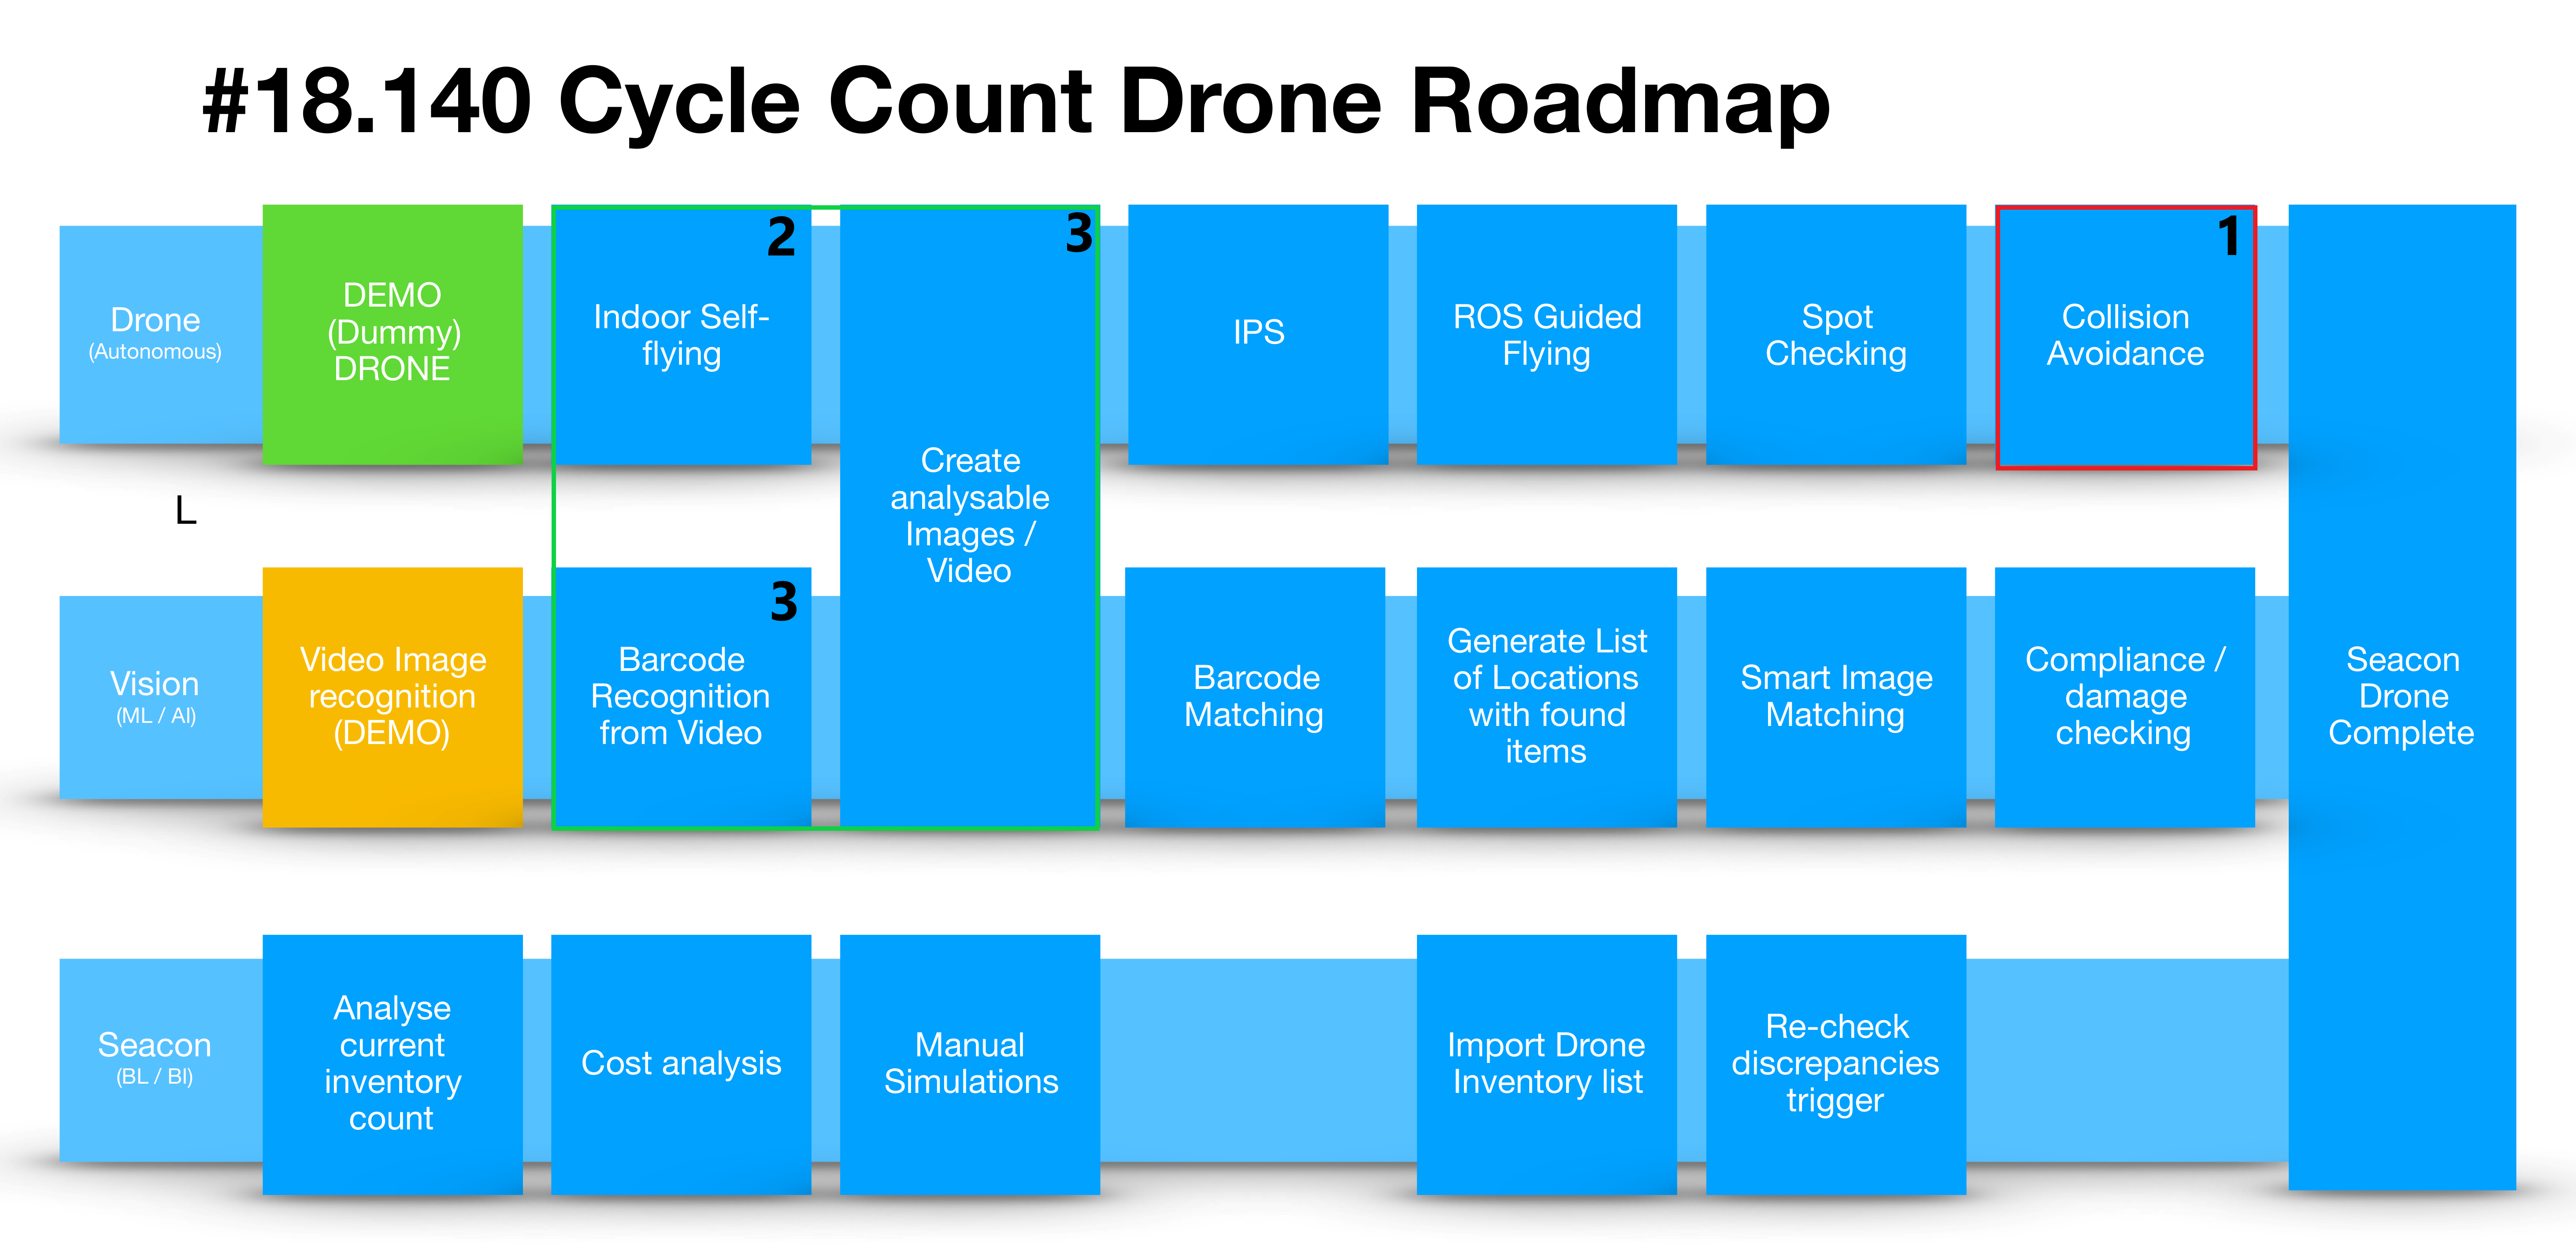
\includegraphics[width=\linewidth]{img/seacon_roadmap.png}
	\caption{Roadmap of the cycle count drone project.}
	\label{fig:roadmap}
\end{figure}
\pagebreak

\noindent
Due to the image size, the states the drone will traverse through can be found in appendix \ref{app:drone_states}. To display how tasks will eventually integrate, the scanning of barcodes has also been added. At a later point in time, however, this could be replaced with a task state containing all the specific tasks as substates.
\section{Reporting Structure}
\label{sec:structure}
The following subjects will come to pass: Firstly, the drone simulation is discussed. Secondly, the research done around the collision avoidance solution up until now will be described. Thirdly, the general adjustments made will be mentioned. Fourthly and finally, a self-reflection is given. All parts (aside from the general adjustments) will also include their respective future plans.